%% REGISTRY: Definition n | Lemma n | Theorem n | source | eq. numbers
%%  Def 1  Binomial tree, risk-neutral price | Tree.ipynb cells 17, 19, 33, 37-38; coding cell 8 | eq:pq, eq:V0, eq:VN
%%  Def 2  Balanced tree                     | Tree.ipynb cell 56; coding cells 12-14             | eq:bal
%%  Def 3  Flat interest rate                | coding cell 20                                     | eq:flat
%%  Thm 1  Vega of the BS call               | Homework 1 (HW 2/2); Lesson 3 cell 49               | eq:vega
%%  Lem 1  Balanced down step                | from Def 1, Def 2                                  | eq:down
%%  Lem 2  Mean and spread of one step       | from Def 1, Lem 1                                  | eq:mean, eq:std
%%  Lem 3  One-step balanced price           | from Def 1, Lem 1                                  | eq:one, eq:range
\RequirePackage{fix-cm}
\documentclass[11pt,a4paper]{article}
\usepackage[utf8]{inputenc}
\usepackage[margin=2cm]{geometry}
\usepackage{amsmath,amssymb,mathtools}
\usepackage{booktabs,array}
\usepackage[most]{tcolorbox}
\usepackage{enumitem}
\setlist[itemize]{itemsep=1pt, topsep=2pt, label=$\bullet$}
\setlist[enumerate]{itemsep=1pt, topsep=2pt}
\usepackage{listings}
\usepackage{tikz}
\usepackage{pgfplots}
\pgfplotsset{compat=1.18}
% ---- matplotlib look for the plots drawn by LaTeX (no image files needed)
\definecolor{tabblue}{HTML}{1F77B4}\definecolor{taborange}{HTML}{FF7F0E}
\definecolor{tabgreen}{HTML}{2CA02C}\definecolor{tabred}{HTML}{D62728}
\pgfplotsset{mpl/.style={scale only axis, axis line style={black,line width=0.8pt},
  tick style={black,line width=0.8pt}, tick align=outside, xtick pos=bottom, ytick pos=left,
  major tick length=3.5pt, tick label style={font=\fontsize{10}{12}\selectfont\sffamily},
  legend cell align=left, legend style={draw=black!20, rounded corners=2pt, fill=white, fill opacity=0.8, text opacity=1},
  legend image code/.code={\draw[#1] (0pt,0pt) -- (22pt,0pt);}},
  mplgrid/.style={grid=major, major grid style={black!30, line width=0.8pt, dash pattern=on 2.96pt off 1.28pt}}}
\tikzset{mpldash/.style={dash pattern=on 3.7pt off 1.6pt}, mpldot/.style={dash pattern=on 1pt off 1.65pt}}
\usepackage{caption}
\usepackage{hyperref}
\hypersetup{colorlinks=true,linkcolor=black,citecolor=black,urlcolor=black,
  pdftitle={Financial Processes -- Homework 2: calibrator for Tree, part 1 (background)},pdfauthor={Carlos Chipantiza}}
\usepackage{needspace}
\frenchspacing
\emergencystretch=3em

\definecolor{DefBlue}{RGB}{16,64,120}
\definecolor{LemRed}{RGB}{170,30,40}
\definecolor{ThmPurple}{RGB}{95,40,130}
\definecolor{AnsGreen}{RGB}{20,120,70}
\definecolor{CodeGray}{RGB}{110,110,110}
\definecolor{FIX}{RGB}{20,120,70}

\newcounter{defn}\newcounter{lemn}\newcounter{thmn}
\newtcolorbox{defbox}[1]{enhanced,colback=white,colframe=DefBlue,boxrule=0.8pt,arc=1mm,left=2mm,right=2mm,top=1.5mm,bottom=1.5mm,
  before upper={\refstepcounter{defn}\noindent\textbf{Definition \thedefn} (#1).\par\smallskip}}
\newtcolorbox{lembox}[1]{enhanced,colback=white,colframe=LemRed,boxrule=0.8pt,arc=1mm,left=2mm,right=2mm,top=1.5mm,bottom=1.5mm,
  before upper={\refstepcounter{lemn}\noindent\textbf{Lemma \thelemn} (#1).\par\smallskip}}
\newtcolorbox{thmbox}[1]{enhanced,colback=white,colframe=ThmPurple,boxrule=0.8pt,arc=1mm,left=2mm,right=2mm,top=1.5mm,bottom=1.5mm,
  before upper={\refstepcounter{thmn}\noindent\textbf{Theorem \thethmn} (#1).\par\smallskip}}
\newtcolorbox{ansboxenv}{enhanced,colback=AnsGreen!6,colframe=AnsGreen,boxrule=0.8pt,arc=1mm,left=2mm,right=2mm,top=1.5mm,bottom=1.5mm}
\newcommand{\ansbox}[1]{\begin{ansboxenv}#1\end{ansboxenv}}
\newcommand{\subhead}[1]{\par\medskip\noindent{\large\bfseries #1}\par\smallskip\noindent\ignorespaces}

% ---- code that can be copied from the PDF and pasted into Python:
% every space is a real character (an invisible glyph mapped to U+0020), no line
% numbers, no line breaks inside a line, straight quotes.
\input{glyphtounicode}
\pdfglyphtounicode{visiblespace}{0020}
\pdfgentounicode=1
\makeatletter
\def\lst@visiblespace{{\color{white}\char32}}
\makeatother
\lstdefinestyle{py}{language=Python,basicstyle=\ttfamily\footnotesize,keywordstyle=\color{DefBlue},
  commentstyle=\color{CodeGray},stringstyle=\color{black},showspaces=true,showstringspaces=false,
  frame=single,rulecolor=\color{CodeGray},numbers=none,
  breaklines=false,columns=fixed,basewidth=0.5em,keepspaces=true,tabsize=4,xleftmargin=0.4em,framexleftmargin=0.4em,
  captionpos=t,literate={\$}{{\char36}}1 {'}{{\char13}}1 {`}{{\char18}}1}
\lstdefinestyle{prof}{style=py,basicstyle=\ttfamily\fontsize{6.6}{7.8}\selectfont}
\lstdefinestyle{pysmall}{style=py,basicstyle=\ttfamily\fontsize{7.6}{9}\selectfont}
\lstdefinestyle{out}{basicstyle=\ttfamily\footnotesize,columns=fixed,basewidth=0.5em,showspaces=true,
  frame=leftline,framerule=1.2pt,rulecolor=\color{FIX},numbers=none,xleftmargin=0.8em,framexleftmargin=0.4em,
  breaklines=false,captionpos=t}
\captionsetup[lstlisting]{labelformat=empty,font={footnotesize,sf},justification=raggedright,singlelinecheck=false,skip=2pt}
\newcommand{\Et}{\tilde{E}}

\begin{document}
\noindent Name: Carlos Chipantiza \hfill Neptun code: EACN90\\
\noindent Financial Processes (BMETE95MM14), BME, Fall 2026 \hfill course id: 54932fw\\[2pt]
{\large\textbf{Homework 2: Implement calibrator for Tree. Part 1: Background}}\\[2pt]
\noindent\rule{\textwidth}{0.4pt}

\noindent\textbf{Remark.} The results used are stated in boxes and cited by number together with the displayed equation. Each one is a result of the lecture on the binomial tree (notebooks \texttt{Tree.ipynb} and \texttt{Binomial\_tree\_coding.ipynb}; the cell is given in the box), a result of Homework~1, or it is proved right after its box. The code of the lecture is used unchanged; the new code is short and marked as such. All the code of this part is in the notebook \texttt{2\_HW\_EXE\_1} (same order as here), and in the files \texttt{prof\_tree.py} (lecture code), \texttt{bg\_functions.py} (new code) and \texttt{plotter.py} (Homework~1). The running example is the one of the lecture: $S_0=K=1$, $T=1$ year, one-year discount factor $0.95$.

\vspace{0.5 cm}
\subhead{The assignment.}
\emph{Background: In the Black--Scholes model volatility is a key parameter that determines option price. In a Balanced Binomial Tree (i.e.\ risk-neutral up step probability $=0.5$, risk-neutral down step probability $=0.5$) the same role is played by step size: higher step is like higher volatility, it results in higher option prices. Also, there is a 1-1 correspondence between step size and price if all other parameters are fixed.}

\noindent This part checks the background, which is what makes the calibration of the Task possible. It contains three claims:
\begin{itemize}
\item \textbf{(C1)} in a balanced tree the step size plays the role of the volatility;
\item \textbf{(C2)} a higher step gives a higher call price;
\item \textbf{(C3)} with all other parameters fixed, step size and price determine each other (1--1).
\end{itemize}
The Task (the \texttt{calibrate} method) will be part 2.

% ============================================================================ results
\subhead{Results used.}

\begin{defbox}{Binomial tree and risk-neutral price; \texttt{Tree.ipynb}, cells 17, 19, 33, 37--38}
In one step the stock goes from $S_0$ to $S_1(U)=uS_0$ or $S_1(D)=dS_0$, and money in the money market grows by the factor $1+r$, with
\[
d<1+r<u .
\]
The risk-neutral probabilities are
\begin{equation}\label{eq:pq}
\tilde p=\frac{1+r-d}{u-d},\qquad \tilde q=1-\tilde p ,
\end{equation}
the price of an option with payoff $V_1$ is
\begin{equation}\label{eq:V0}
V_0=\frac{1}{1+r}\,\Et(V_1)=\frac{1}{1+r}\bigl(\tilde p\,V_1(U)+\tilde q\,V_1(D)\bigr),
\end{equation}
and in a tree with $N$ steps (spot tree $S_{t,i}$, $t=0,\dots,N$, $i=0,\dots,t$)
\begin{equation}\label{eq:VN}
V_0=\frac{1}{(1+r)^N}\,\Et(V_N).
\end{equation}
In the code of \texttt{Binomial\_tree\_coding.ipynb} (cell 8) the parameter is the discount factor of one step, $DF=1/(1+r)$; the leaves are multiplied by $DF^N$ and the backward steps use $\tilde p$ and $\tilde q$.
\end{defbox}

\begin{defbox}{Balanced tree; \texttt{Tree.ipynb}, cell 56; \texttt{Binomial\_tree\_coding.ipynb}, cells 12--14}
A binomial tree is \emph{balanced} if
\begin{equation}\label{eq:bal}
\tilde p=\tilde q=\tfrac12 .
\end{equation}
The \emph{up step} is the factor $u$ (\texttt{spot\_mult\_up}); in the balanced tree the down step $d$ (\texttt{spot\_mult\_down}) is computed from $u$ by \texttt{calcBalancedDownStep}.
\end{defbox}

\begin{defbox}{Flat interest rate; \texttt{Binomial\_tree\_coding.ipynb}, cell 20}
For a maturity of $T$ years and $N$ steps, each step is $\Delta t=T/N$ years long, and the discount factor of one step is the one-year discount factor $DF_1$ to the power $\Delta t$:
\begin{equation}\label{eq:flat}
DF=DF_1^{\,\Delta t},\qquad \Delta t=\frac{T}{N}.
\end{equation}
Then $DF^N=DF_1^{\,T}$ for every $N$: ``discount factors have to be scaled to keep interest rate fixed''.
\end{defbox}

\begin{thmbox}{Vega of the Black--Scholes call; Homework 1, HW 2/2 (Lesson 3, cell 49)}
The Black--Scholes call price $c$ has
\begin{equation}\label{eq:vega}
\mathcal V=\frac{\partial c}{\partial\sigma}=S_0\,N'(d_1)\sqrt T>0 ,
\end{equation}
so $c$ is strictly increasing in the volatility $\sigma$. In Homework 1 the pricer \texttt{black\_scholes\_eur\_call} (HW 2/2, new version) returns $c$ and, with \texttt{return\_greeks=True}, also $\mathcal V$.
\end{thmbox}

\subhead{The code of the lecture.} Cells 3, 5, 8 and 13 of \texttt{Binomial\_tree\_coding.ipynb}, unchanged (with the imports of cell 1):
\par\smallskip\noindent\begin{minipage}{\linewidth}\begin{lstlisting}[style=prof,title={lecture code (\texttt{prof\_tree.py})}]
import numpy as np
from scipy.optimize import minimize
from collections.abc import Callable


def european_call_payoff(S: float, K: float) -> float:
    return max(S-K, 0.0)


def create_spot_tree(spot: float, spot_mult_up: float, spot_mult_down: float, steps: int) -> list[list[float]]:
    previous_level = [spot]
    tree = [previous_level]
    for _ in range(steps):
        new_level = [s * spot_mult_down for s in previous_level]
        new_level += [previous_level[-1] * spot_mult_up]
        tree += [new_level]
        previous_level = new_level
    return tree


def create_discounted_price_tree(spot_tree: list[list[float]], discount_factor: float, K: float, diag: int = 0) -> list[list[float]]:
    spot = spot_tree[0][0]
    spot_mult_up = spot_tree[1][-1]
    spot_mult_down = spot_tree[1][0]
    p_up = ((1 / discount_factor - spot_mult_down) /
                   (spot_mult_up - spot_mult_down))
    p_down = 1 - p_up
    steps = len(spot_tree) - 1
    continuation_value_tree = [[np.nan for _ in level] for level in spot_tree]
    if diag > 0:
        print("risk-neutral measure: ")
        print(('%.3f' % p_up, '%.3f' % p_down))
        # init delta tree
        delta_tree = [[np.nan for _ in level] for level in spot_tree[:-1]] #delta makes no sense for leaves
    # going backwards, payoff is known in leaves
    for i in range(len(spot_tree[-1])):
        spot = spot_tree[-1][i]
        discounted_continuation_value = discount_factor**(steps) * european_call_payoff(spot, K)
        continuation_value_tree[-1][i] = discounted_continuation_value
    for step in range(steps - 1, -1, -1):
        for i in range(len(spot_tree[step])):
            continuation_value_tree[step][i] = p_up * continuation_value_tree[step + 1][i] + \
                                            p_down * continuation_value_tree[step + 1][i + 1]
            if diag > 0:
                delta_tree[step][i] = ((continuation_value_tree[step + 1][i] - continuation_value_tree[step + 1][i + 1]) 
                                       / (spot_tree[step + 1][i] - spot_tree[step + 1][i + 1]))
    if diag > 0:
        print("delta: ")
        delta_tree_readable = [['%.3f' % e for e in n] for n in delta_tree]
        print(delta_tree_readable)
    return continuation_value_tree


def calcBalancedDownStep(spot_mult_up: float, discount_factor: float) -> (float, float):
    return spot_mult_up - 2 * (spot_mult_up - 1 / discount_factor)
\end{lstlisting}\end{minipage}\par\smallskip

\begin{lembox}{Balanced down step; from Definitions~1 and 2}
The tree is balanced, \eqref{eq:bal}, exactly when
\begin{equation}\label{eq:down}
d=\frac{2}{DF}-u ,
\end{equation}
which is what \texttt{calcBalancedDownStep} returns: $u-2\,(u-1/DF)=2/DF-u$. The condition $d<1+r<u$ of Definition~1 then means $u>1/DF$, and $d>0$ means $u<2/DF$; so the up step can be any
\[
u\in\Bigl(\frac1{DF},\ \frac2{DF}\Bigr).
\]
\end{lembox}

\noindent\textit{Proof.} With $1+r=1/DF$, we set $\tilde p$ of \eqref{eq:pq} equal to $\tfrac12$ and solve for $d$ by levels:
\begin{align*}
\frac{1/DF-d}{u-d} &= \frac12 && \text{(Definition~1, \eqref{eq:pq}; Definition~2, \eqref{eq:bal})}\\
2\Bigl(\frac1{DF}-d\Bigr) &= u-d && \text{(multiply by $2(u-d)>0$)}\\
d &= \frac2{DF}-u. && \text{(collect $d$)}
\end{align*}
Then $d<1/DF$ is $2/DF-u<1/DF$, that is $u>1/DF$; and $d>0$ is $u<2/DF$. \hfill$\square$



\vspace{0.8 cm}
\subhead{New code.} One function prices the call in a balanced tree with the lecture code; the second one gives the up step for a chosen \emph{tree volatility} (introduced in (C1) below):
\par\smallskip\noindent\begin{minipage}{\linewidth}\begin{lstlisting}[style=py,title={new code (\texttt{bg\_functions.py})}]
def balanced_tree_call_price(spot: float, strike: float, maturity: float, steps: int,
                             df_annual: float, spot_mult_up: float) -> float:
    """Price of a European call in a Balanced Binomial Tree (p_up = p_down = 0.5)."""
    discount_factor = df_annual ** (maturity / steps)     # per step: keeps the rate flat
    spot_mult_down = calcBalancedDownStep(spot_mult_up, discount_factor)
    spot_tree = create_spot_tree(spot, spot_mult_up, spot_mult_down, steps)
    price_tree = create_discounted_price_tree(spot_tree, discount_factor, strike)
    return price_tree[0][0]


def up_step_from_tree_vol(sigma_tree: float, maturity: float, steps: int,
                          df_annual: float) -> float:
    """Up step u with step size u - 1/DF = sigma_tree * sqrt(dt)."""
    dt = maturity / steps
    discount_factor = df_annual ** dt
    return 1 / discount_factor + sigma_tree * np.sqrt(dt)
\end{lstlisting}\end{minipage}\par\smallskip

% ============================================================================ C1
\subhead{(C1) The step size plays the role of the volatility.}

\begin{lembox}{Mean and spread of one step of a balanced tree; from Definition~1 and Lemma~1}
In one step of a balanced tree the stock is multiplied by $X=S_{t+1}/S_t$, which is $u$ or $d$ with risk-neutral probability $\tfrac12$ each. Then
\begin{equation}\label{eq:mean}
\Et(X)=\frac1{DF},
\end{equation}
\begin{equation}\label{eq:std}
\sqrt{\Et\bigl((X-\Et X)^2\bigr)}=u-\frac1{DF}.
\end{equation}
\end{lembox}

\noindent\textit{Proof.} By Lemma~1, \eqref{eq:down}, $d=2/DF-u$, so
\begin{align*}
\Et(X) &= \tfrac12\,u+\tfrac12\,d\\
&= \tfrac12\Bigl(u+\frac2{DF}-u\Bigr)\\
&= \frac1{DF}.
\end{align*}
Hence $u-\Et X=u-1/DF$ and $d-\Et X=1/DF-u=-(u-1/DF)$: both values are at the same distance $u-1/DF$ from the mean, and
\begin{align*}
\Et\bigl((X-\Et X)^2\bigr) &= \tfrac12\Bigl(u-\frac1{DF}\Bigr)^2+\tfrac12\Bigl(u-\frac1{DF}\Bigr)^2\\
&= \Bigl(u-\frac1{DF}\Bigr)^2 .
\end{align*}
Since $u>1/DF$ (Lemma~1), the square root is $u-1/DF$. \hfill$\square$

\noindent So in a balanced tree the mean of a step is fixed by the interest rate, \eqref{eq:mean}, and the up step only changes the spread around it, \eqref{eq:std}. We call
\[
h=u-\frac1{DF}
\]
the \emph{step size}: it is the standard deviation of one step, which in the Black--Scholes model is about $\sigma\sqrt{\Delta t}$. To compare trees with different numbers of steps with each other and with $\sigma$, we use the \emph{tree volatility}
\[
\sigma_{\text{tree}}=\frac{h}{\sqrt{\Delta t}}=\frac{u-1/DF}{\sqrt{\Delta t}},
\qquad\text{that is,}\qquad u=\frac1{DF}+\sigma_{\text{tree}}\sqrt{\Delta t}
\]
(function \texttt{up\_step\_from\_tree\_vol}). The lecture (cell 20) chooses the up step from a volatility $\sigma$ as $u=\exp\bigl((r-\sigma^2/2)\Delta t+\sigma\sqrt{\Delta t}\bigr)$; for $\sigma=0.1$ and $7$ steps per year this gives $\sigma_{\text{tree}}\approx0.1002$, almost the same number. The check:
\par\smallskip\noindent\begin{minipage}{\linewidth}\begin{lstlisting}[style=py,title={check of (C1)}]
# (C1) one step of a balanced tree: mean and standard deviation of the factor S_{n+1}/S_n
discount_factor = 0.95
for spot_mult_up in [1.10, 1.20, 1.40]:
    spot_mult_down = calcBalancedDownStep(spot_mult_up, discount_factor)
    p_up = (1 / discount_factor - spot_mult_down) / (spot_mult_up - spot_mult_down)
    mean = p_up * spot_mult_up + (1 - p_up) * spot_mult_down
    std = np.sqrt(p_up * (spot_mult_up - mean)**2 + (1 - p_up) * (spot_mult_down - mean)**2)
    print(f"u = {spot_mult_up:.2f}  d = {spot_mult_down:.4f}  p_up = {p_up:.2f}  "
          f"mean = {mean:.4f}  std = {std:.4f}  u - 1/DF = {spot_mult_up - 1/discount_factor:.4f}")

# the up step of the lecture (cell 20): sigma = 0.1, 7 steps per year
steps_per_year = 7
dt = 1 / steps_per_year
discount_factor = 0.95 ** dt
spot_mult_up = np.exp((0.05 - 0.5 * 0.1 ** 2) * dt + 0.1 * np.sqrt(dt))
print(f"lecture: u = {spot_mult_up:.6f}  step size u - 1/DF = {spot_mult_up - 1/discount_factor:.6f}"
      f"  sigma_tree = {(spot_mult_up - 1/discount_factor) / np.sqrt(dt):.4f}")
\end{lstlisting}
\begin{lstlisting}[style=out,title={output}]
u = 1.10  d = 1.0053  p_up = 0.50  mean = 1.0526  std = 0.0474  u - 1/DF = 0.0474
u = 1.20  d = 0.9053  p_up = 0.50  mean = 1.0526  std = 0.1474  u - 1/DF = 0.1474
u = 1.40  d = 0.7053  p_up = 0.50  mean = 1.0526  std = 0.3474  u - 1/DF = 0.3474
lecture: u = 1.045218  step size u - 1/DF = 0.037863  sigma_tree = 0.1002
\end{lstlisting}\end{minipage}\par\smallskip
In every case $\tilde p=0.5$, the mean is $1/DF\approx1.0526$ and the standard deviation equals $u-1/DF$, as Lemma~2 says.

% ============================================================================ C2, C3 one step
\subhead{(C2) and (C3) for a one-step tree.}

\begin{lembox}{Price of a call in a one-step balanced tree; from Definition~1 and Lemma~1}
Let $N=1$, $u\in(1/DF,2/DF)$, and let the strike satisfy $0<K<2S_0/DF$. Then the call price is
\begin{equation}\label{eq:one}
V_0(u)=\frac{DF}{2}\Bigl((uS_0-K)^+ +\bigl((\tfrac2{DF}-u)S_0-K\bigr)^+\Bigr).
\end{equation}
With $u^*=\max\{K/S_0,\ 2/DF-K/S_0\}$, the price is constant, equal to $(S_0-DF\,K)^+$, for $u\le u^*$, and
\[
V_0(u)=\frac{DF}{2}\,(uS_0-K)\qquad\text{for } u^*\le u<\frac2{DF},
\]
which is strictly increasing in $u$. Hence $u\mapsto V_0(u)$ is a bijection
\begin{equation}\label{eq:range}
\Bigl[u^*,\ \frac2{DF}\Bigr)\ \longrightarrow\ \Bigl[(S_0-DF\,K)^+,\ S_0-\frac{DF\,K}{2}\Bigr).
\end{equation}
\end{lembox}

\noindent\textit{Proof.} By Definition~1, \eqref{eq:V0}, with $\tilde p=\tilde q=\tfrac12$, $1/(1+r)=DF$, the call payoffs $V_1(U)=(uS_0-K)^+$, $V_1(D)=(dS_0-K)^+$ and $d=2/DF-u$ (Lemma~1, \eqref{eq:down}) we get \eqref{eq:one}. Now $uS_0>K$ exactly when $u>K/S_0$, and $dS_0<K$ exactly when $u>2/DF-K/S_0$.
\begin{itemize}
\item If $u\ge u^*$: the up leaf is at or above $K$ and the down leaf at or below $K$, so $V_0=\frac{DF}{2}(uS_0-K)$, a line with slope $DF\,S_0/2>0$.
\item If $u\le u^*$: then $uS_0\le K$ or $dS_0\ge K$, and since $dS_0<uS_0$, both leaves are on the same side of $K$. If both are at or above $K$, so is their mean $\frac{u+d}{2}S_0=S_0/DF$, hence $S_0-DF\,K\ge0$, and by $u+d=2/DF$
\[
V_0=\tfrac{DF}2(uS_0+dS_0-2K)=\tfrac{DF}{2}\bigl(\tfrac{2S_0}{DF}-2K\bigr)=S_0-DF\,K .
\]
If both are at or below $K$, then $S_0/DF\le K$ and $V_0=0$. In both cases $V_0=(S_0-DF\,K)^+$, which does not depend on $u$.
\end{itemize}
The value at $u^*$ is $(S_0-DF\,K)^+$ from both formulas, and the line tends to $\frac{DF}2\bigl(\frac{2S_0}{DF}-K\bigr)=S_0-\frac{DF\,K}2$ as $u\to2/DF$. A continuous, strictly increasing function on an interval is a bijection onto the interval between its end values, which gives \eqref{eq:range}. \hfill$\square$

\noindent The check computes the price with the lecture code for $400$ up steps $u$ and three strikes (in the money, at the money forward $K=S_0/DF$ as in cell 16 of the lecture, out of the money), compares it with \eqref{eq:one}, and draws Figure~\ref{fig:one} with the plotter of Homework~1 (HW 2/1, \texttt{plotter.py}):
\par\smallskip\noindent\begin{minipage}{\linewidth}\begin{lstlisting}[style=pysmall,title={check of (C2) and (C3), one step}]
# (C2), (C3) one-step tree: price against the up step u, for three strikes
spot, maturity, df_annual = 1.0, 1.0, 0.95
u_grid = np.linspace(1 / df_annual + 1e-6, 2 / df_annual - 1e-6, 400)
strikes = [0.9, spot / df_annual, 1.2]                  # in the money, ATM forward, out of the money
prices = [[balanced_tree_call_price(spot, K, maturity, 1, df_annual, u) for u in u_grid]
          for K in strikes]

# the formula of Lemma 3 gives the same prices
for K, p in zip(strikes, prices):
    d_grid = 2 / df_annual - u_grid
    formula = df_annual / 2 * (np.maximum(u_grid * spot - K, 0) + np.maximum(d_grid * spot - K, 0))
    u_star = max(K / spot, 2 / df_annual - K / spot)
    print(f"K = {K:.4f}: max |tree - formula| = {np.max(np.abs(np.array(p) - formula)):.1e},"
          f"  u* = {u_star:.4f},  price range [{p[0]:.4f}, {p[-1]:.4f}]")

fig, ax = my_plotter(u_grid, prices,
                     layout={"title": "One-step balanced tree: call price against the up step",
                             "x_label": "up step $u$", "y_label": "call price", "hline": None,
                             "grid": True, "figsize": (8, 4), "title_fontsize": 13,
                             "label_fontsize": 11, "legend_fontsize": 10, "linewidth": 2},
                     names=["K = 0.9", "K = 1/0.95 (ATM forward)", "K = 1.2"])
\end{lstlisting}
\begin{lstlisting}[style=out,title={output}]
K = 0.9000: max |tree - formula| = 2.8e-17,  u* = 1.2053,  price range [0.1450, 0.5725]
K = 1.0526: max |tree - formula| = 0.0e+00,  u* = 1.0526,  price range [0.0000, 0.5000]
K = 1.2000: max |tree - formula| = 0.0e+00,  u* = 1.2000,  price range [0.0000, 0.4300]
\end{lstlisting}\end{minipage}\par\smallskip
The lecture code and \eqref{eq:one} agree to rounding; $u^*$ and the price range are the ones of Lemma~3: for $K=0.9$, $u^*=2/0.95-0.9\approx1.2053$ and the range is $[1-0.95\cdot0.9,\ 1-0.95\cdot0.45)=[0.1450,\ 0.5725)$.

\begin{figure}[!ht]
\centering
\resizebox{0.72\textwidth}{!}{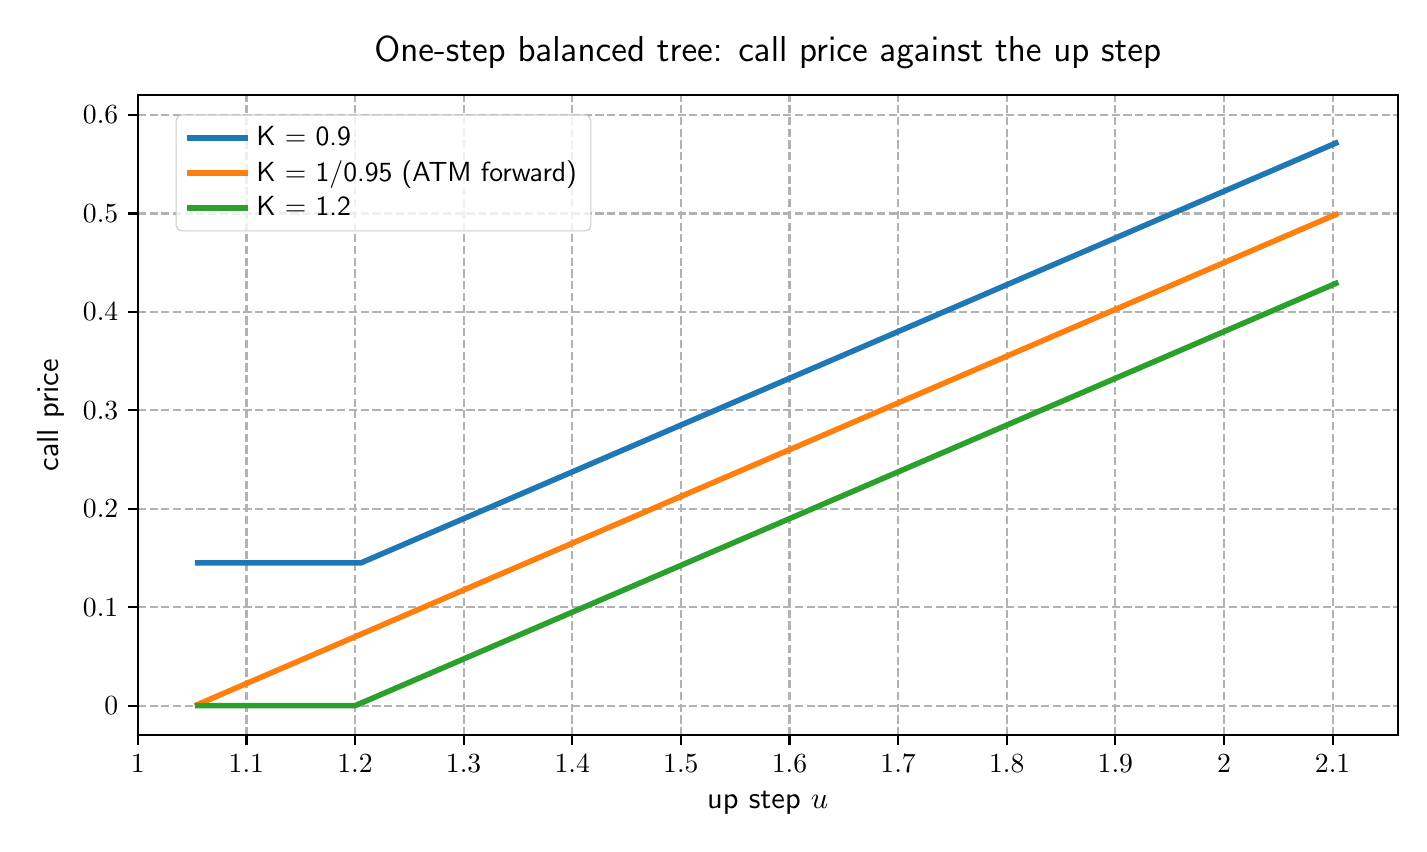
\begin{tikzpicture}
\begin{axis}[mpl, mplgrid, width=6.3in, height=3.2in, xmin=1.0, xmax=2.16, ymin=-0.03, ymax=0.62,
  title={\fontsize{13}{15}\selectfont\sffamily One-step balanced tree: call price against the up step},
  xlabel={\fontsize{11}{13}\selectfont\sffamily up step $u$}, ylabel={\fontsize{11}{13}\selectfont\sffamily call price},
  legend pos=north west, legend style={font=\fontsize{10}{12}\selectfont\sffamily}]
\addplot[tabblue, line width=2pt] coordinates {(1.0526,0.1450) (1.2053,0.1450) (2.1053,0.5725)};
\addlegendentry{K = 0.9}
\addplot[taborange, line width=2pt] coordinates {(1.0526,0.0000) (2.1053,0.5000)};
\addlegendentry{K = 1/0.95 (ATM forward)}
\addplot[tabgreen, line width=2pt] coordinates {(1.0526,0.0000) (1.2000,0.0000) (2.1053,0.4300)};
\addlegendentry{K = 1.2}
\end{axis}
\end{tikzpicture}}
\caption{Output of the one-step check ($S_0=1$, $T=1$, $DF=0.95$). Each price is flat up to $u^*$ and then increases linearly; for the at-the-money-forward strike $u^*=1/DF$, so it increases on the whole range.}
\label{fig:one}
\end{figure}

% ============================================================================ C2, C3 N steps
\subhead{(C2) and (C3) for several steps, and the comparison with Black--Scholes.}
For $N=1,2,5,50$ steps we price the call $S_0=K=1$, $T=1$ with the flat rate of Definition~3 (one-year discount factor $0.95$), for tree volatilities from $0.005$ to $0.6$. Next to it, the Black--Scholes price of Homework~1 with the same rate, $r=-\ln0.95$, and $\sigma=\sigma_{\text{tree}}$:
\par\smallskip\noindent\begin{minipage}{\linewidth}\begin{lstlisting}[style=pysmall,title={check of (C2) and (C3), several steps}]
# (C2), (C3) N-step trees against the tree volatility, and the Black-Scholes price of Homework 1
spot, strike, maturity, df_annual = 1.0, 1.0, 1.0, 0.95
r = -np.log(df_annual)                                   # the same flat interest rate
sigma_grid = np.linspace(0.005, 0.6, 120)
curves, names = [], []
for steps in [1, 2, 5, 50]:
    curves.append([balanced_tree_call_price(spot, strike, maturity, steps, df_annual,
                                            up_step_from_tree_vol(s, maturity, steps, df_annual))
                   for s in sigma_grid])
    names.append(f"tree, N = {steps}")
curves.append([black_scholes_eur_call(r=r, T=maturity, S0=spot, sigma=s, K=strike)[0]
               for s in sigma_grid])         # one sigma at a time (assert sigma > 0)
names.append("Black-Scholes (Homework 1)")

for s in [0.1, 0.2, 0.3]:
    i = np.argmin(np.abs(sigma_grid - s))
    print(f"sigma = {sigma_grid[i]:.3f}: " + "  ".join(f"{c[i]:.4f}" for c in curves))
print("increasing:", [bool(np.all(np.diff(c) >= -1e-12)) for c in curves])

fig, ax = my_plotter(sigma_grid, curves,
                     layout={"title": "Call price against the tree volatility (S0 = K = 1, T = 1)",
                             "x_label": "tree volatility $(u - 1/DF)/\\sqrt{\\Delta t}$, or $\\sigma$",
                             "y_label": "call price", "hline": None, "grid": True, "figsize": (8, 4),
                             "title_fontsize": 13, "label_fontsize": 11, "legend_fontsize": 10,
                             "linewidth": 2, "linestyles": ["-", "-", "-", "-", "--"],
                             "colors": ["tab:blue", "tab:orange", "tab:green", "tab:red", "black"]},
                     names=names)
\end{lstlisting}
\begin{lstlisting}[style=out,title={output (columns: N = 1, 2, 5, 50, Black-Scholes)}]
sigma = 0.100: 0.0725  0.0708  0.0671  0.0690  0.0689
sigma = 0.200: 0.1200  0.1017  0.1076  0.1055  0.1052
sigma = 0.300: 0.1675  0.1302  0.1480  0.1426  0.1429
increasing: [True, True, True, True, True]
\end{lstlisting}\end{minipage}\par\smallskip
All five curves of Figure~\ref{fig:multi} are increasing (the line \texttt{increasing}), and the tree with $50$ steps is already close to the Black--Scholes price: $0.0690$ against $0.0689$ at $\sigma=0.1$, $0.1055$ against $0.1052$ at $\sigma=0.2$. The Black--Scholes price is strictly increasing in $\sigma$ by Theorem~1, \eqref{eq:vega}; the tree prices behave in the same way in the step size, which is the meaning of (C1)--(C3).

\begin{figure}[!ht]
\centering
\resizebox{0.72\textwidth}{!}{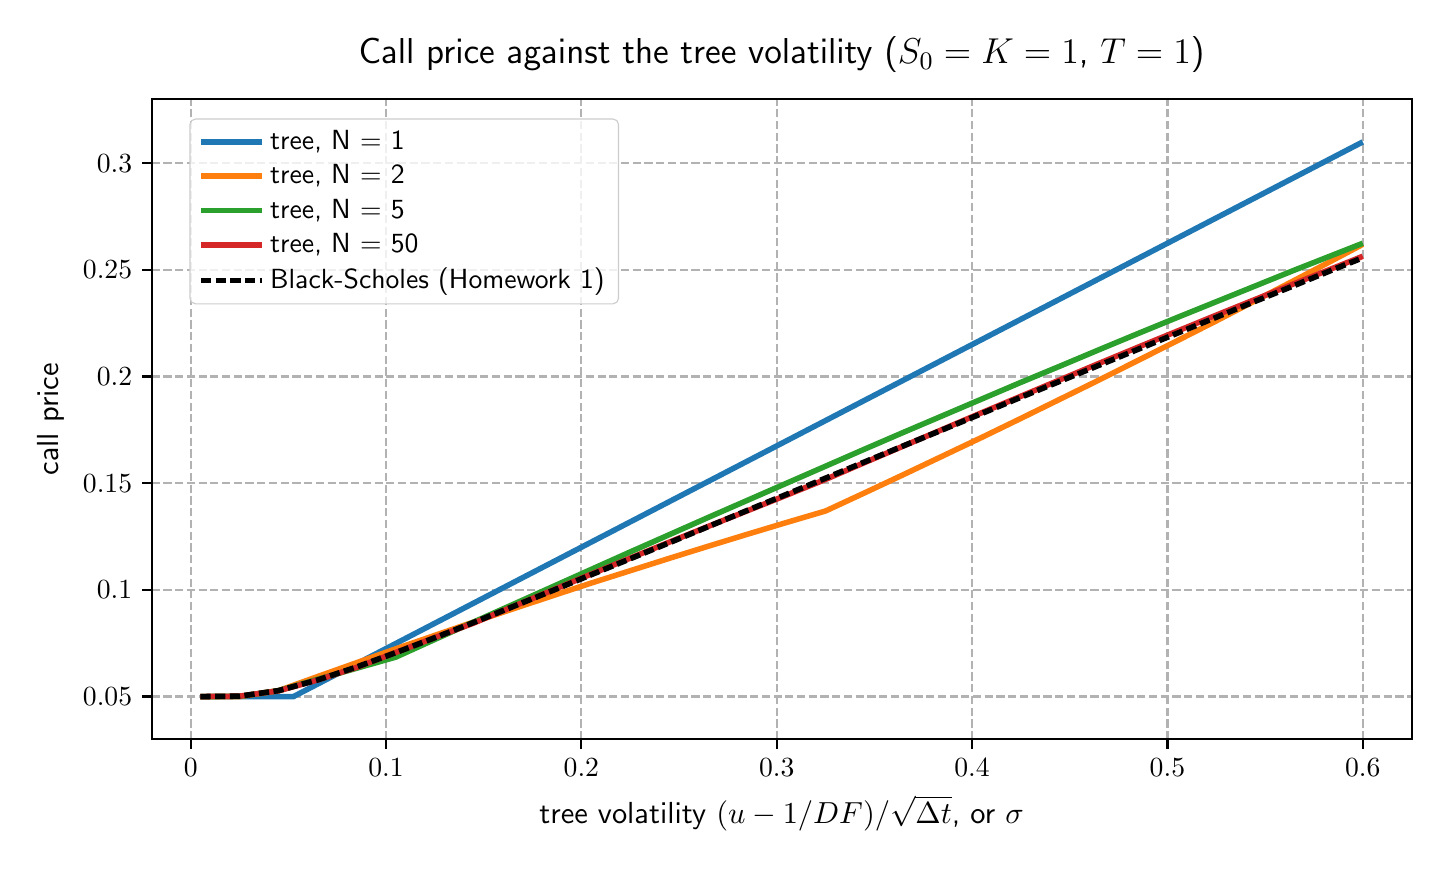
\begin{tikzpicture}
\begin{axis}[mpl, mplgrid, width=6.3in, height=3.2in, xmin=-0.02, xmax=0.625, ymin=0.03, ymax=0.33,
  xtick={0,0.1,0.2,0.3,0.4,0.5,0.6}, ytick={0.05,0.1,0.15,0.2,0.25,0.3},
  xticklabel style={/pgf/number format/fixed}, yticklabel style={/pgf/number format/fixed, /pgf/number format/precision=2},
  title={\fontsize{13}{15}\selectfont\sffamily Call price against the tree volatility ($S_0 = K = 1$, $T = 1$)},
  xlabel={\fontsize{11}{13}\selectfont\sffamily tree volatility $(u - 1/DF)/\sqrt{\Delta t}$, or $\sigma$}, ylabel={\fontsize{11}{13}\selectfont\sffamily call price},
  legend pos=north west, legend style={font=\fontsize{10}{12}\selectfont\sffamily}]
\addplot[tabblue, line width=2pt] coordinates {(0.0050,0.0500) (0.0526,0.0500) (0.6000,0.3100)};
\addlegendentry{tree, N = 1}
\addplot[taborange, line width=2pt] coordinates {(0.0050,0.0500) (0.0250,0.0500) (0.0450,0.0528) (0.0650,0.0594) (0.0850,0.0659) (0.1050,0.0724) (0.1250,0.0787) (0.1450,0.0850) (0.1650,0.0911) (0.1850,0.0972) (0.2050,0.1032) (0.2250,0.1090) (0.2450,0.1148) (0.2650,0.1205) (0.2850,0.1261) (0.3050,0.1316) (0.3250,0.1370) (0.3450,0.1455) (0.3650,0.1541) (0.3850,0.1628) (0.4050,0.1715) (0.4250,0.1804) (0.4450,0.1894) (0.4650,0.1984) (0.4850,0.2076) (0.5050,0.2168) (0.5250,0.2261) (0.5450,0.2356) (0.5650,0.2451) (0.5850,0.2547) (0.6000,0.2620)};
\addlegendentry{tree, N = 2}
\addplot[tabgreen, line width=2pt] coordinates {(0.0050,0.0500) (0.0250,0.0501) (0.0450,0.0528) (0.0650,0.0581) (0.0850,0.0633) (0.1050,0.0685) (0.1250,0.0768) (0.1450,0.0850) (0.1650,0.0932) (0.1850,0.1014) (0.2050,0.1096) (0.2250,0.1178) (0.2450,0.1259) (0.2650,0.1340) (0.2850,0.1420) (0.3050,0.1500) (0.3250,0.1580) (0.3450,0.1660) (0.3650,0.1739) (0.3850,0.1817) (0.4050,0.1895) (0.4250,0.1973) (0.4450,0.2049) (0.4650,0.2126) (0.4850,0.2202) (0.5050,0.2277) (0.5250,0.2351) (0.5450,0.2425) (0.5650,0.2499) (0.5850,0.2571) (0.6000,0.2625)};
\addlegendentry{tree, N = 5}
\addplot[tabred, line width=2pt] coordinates {(0.0050,0.0500) (0.0250,0.0502) (0.0450,0.0527) (0.0650,0.0578) (0.0850,0.0637) (0.1050,0.0707) (0.1250,0.0777) (0.1450,0.0845) (0.1650,0.0922) (0.1850,0.0998) (0.2050,0.1074) (0.2250,0.1149) (0.2450,0.1224) (0.2650,0.1298) (0.2850,0.1371) (0.3050,0.1444) (0.3250,0.1518) (0.3450,0.1597) (0.3650,0.1675) (0.3850,0.1753) (0.4050,0.1831) (0.4250,0.1908) (0.4450,0.1985) (0.4650,0.2062) (0.4850,0.2138) (0.5050,0.2213) (0.5250,0.2288) (0.5450,0.2362) (0.5650,0.2436) (0.5850,0.2509) (0.6000,0.2564)};
\addlegendentry{tree, N = 50}
\addplot[black, line width=2pt, mpldash] coordinates {(0.0050,0.0500) (0.0250,0.0502) (0.0450,0.0528) (0.0650,0.0578) (0.0850,0.0639) (0.1050,0.0706) (0.1250,0.0776) (0.1450,0.0848) (0.1650,0.0922) (0.1850,0.0996) (0.2050,0.1071) (0.2250,0.1146) (0.2450,0.1221) (0.2650,0.1297) (0.2850,0.1373) (0.3050,0.1448) (0.3250,0.1524) (0.3450,0.1600) (0.3650,0.1676) (0.3850,0.1751) (0.4050,0.1827) (0.4250,0.1903) (0.4450,0.1978) (0.4650,0.2053) (0.4850,0.2128) (0.5050,0.2203) (0.5250,0.2278) (0.5450,0.2353) (0.5650,0.2427) (0.5850,0.2502) (0.6000,0.2557)};
\addlegendentry{Black-Scholes (Homework 1)}
\end{axis}
\end{tikzpicture}}
\caption{Output of the check with several steps. The tree prices increase with the step size like the Black--Scholes price increases with $\sigma$, and approach it as $N$ grows.}
\label{fig:multi}
\end{figure}

\ansbox{Hence the background holds, with the step size $h=u-1/DF$ in the role of the volatility:
\begin{itemize}
\item \textbf{(C1)} in a balanced tree $d=2/DF-u$ (Lemma~1); one step has mean $1/DF$, fixed by the interest rate, and standard deviation $u-1/DF$ (Lemma~2), like $\sigma\sqrt{\Delta t}$ in Black--Scholes;
\item \textbf{(C2)} the call price does not decrease when the up step increases (Lemma~3 for one step, Figures~\ref{fig:one} and~\ref{fig:multi}), as the Black--Scholes price increases with $\sigma$ (Theorem~1);
\item \textbf{(C3)} once the strike lies between the leaves, the price is strictly increasing and continuous in $u$, so each attainable price comes from exactly one up step; for one step, \eqref{eq:range}: $u\in[u^*,2/DF)$ and $V_0\in[(S_0-DF\,K)^+,\ S_0-DF\,K/2)$.
\end{itemize}}

\noindent\emph{Comment (to keep in mind for the Task).} The 1--1 correspondence needs two conditions. First, the price is flat for small steps, as long as all leaves are on the same side of the strike (for one step, $u\le u^*$); there the price is the lower bound $(S_0-DF^N K)^+$, and every $u$ in the flat part gives it. Second, not every price can be reached: $d>0$ bounds the up step by $2/DF$, so for one step the price stays below $S_0-DF\,K/2$. So the calibration of part 2 must check that the given price lies in the attainable range and must look for $u$ above the flat part; with more steps the flat part is very short (Figure~\ref{fig:multi}).

\end{document}
